\model{Process Skills}

\begin{minipage}{0.45\textwidth}

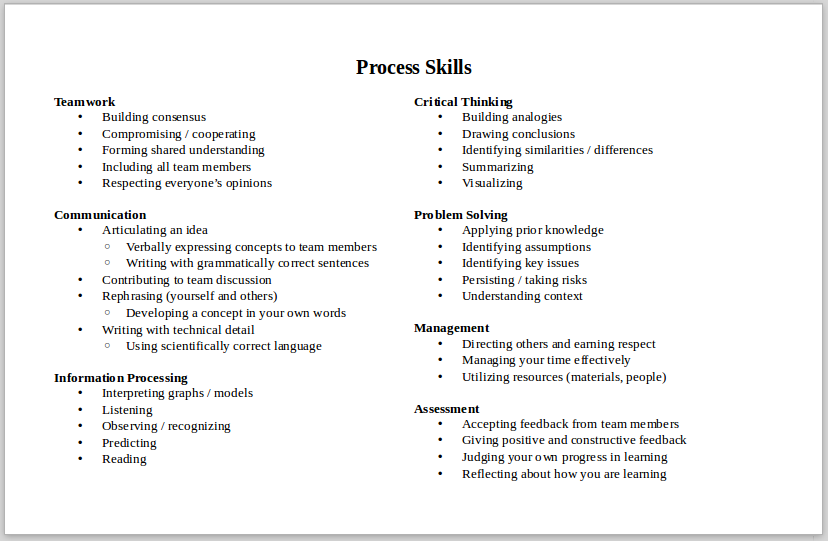
\includegraphics[width=\linewidth]{Meta/process1.png}

\end{minipage}
\hfill
\begin{minipage}{0.5\textwidth}

Your learning team has a new card that is not a role.
It lists and describes the \emph{process skills} that are essential for your ability to construct knowledge.

\end{minipage}


\quest{10 min}


\Q Manager: have each person take turns reading sections of the Process Skills card out loud.
Discuss as a team which skills you would like to focus on today.
Write your top three choices:

\begin{answer}
Teamwork, Problem Solving, Assessment ~ (answers will vary)
\end{answer}


\Q What is a process skill?
As a team, come up with a precise definition.

\begin{answer}[5em]
A skill is ``an ability that has been acquired by training'' (WordNet).
Process skills are what you need to learn in college in addition to content.
\end{answer}


\Q What other knowledge and skills do you expect to learn from this course?
How are they different from process skills?

\begin{answer}[5em]
Answers may include: how to program, how to debug, and the Java language.
These skills are domain-specific; process skills apply to all disciplines.
\end{answer}


\Q Who has the responsibility to ensure that your team thinks about process skills during the activity each week?
How can the other roles support him/her?

\begin{answer}
The reflector should monitor the teams progress with respect to process skills.
But everyone should self assess and point out examples during the activity.
\end{answer}
